\section{Mastodon numerical features.}
\label{FeaturesExplanation}

We describe here how the feature values currently available in Mastodon are calculated. 

\subsection{Spot features.}

\subsubsection{Spot gaussian-filtered intensity.}

This feature has two projections per channel, \textbf{Mean} and \textbf{Std}.
The values are floating point numbers, with the dimension \textbf{Intensity}.

The \textbf{Mean} projections give the average intensity at the center of the spot.
The average is calculated by taking the mean intensity inside the spot, weighted by a gaussian centered on the spot.
The size of the gaussian is adapted to fit into the smallest radius of the spot.
The Figure~\ref{fig:SpotGaussWeights} illustrates the Gaussian weights in the average for several spots.

The \textbf{Std} projections give the standard deviation of these means. 
The standard deviation is also weighted by the Gaussian.

\begin{figure}
    \centering
    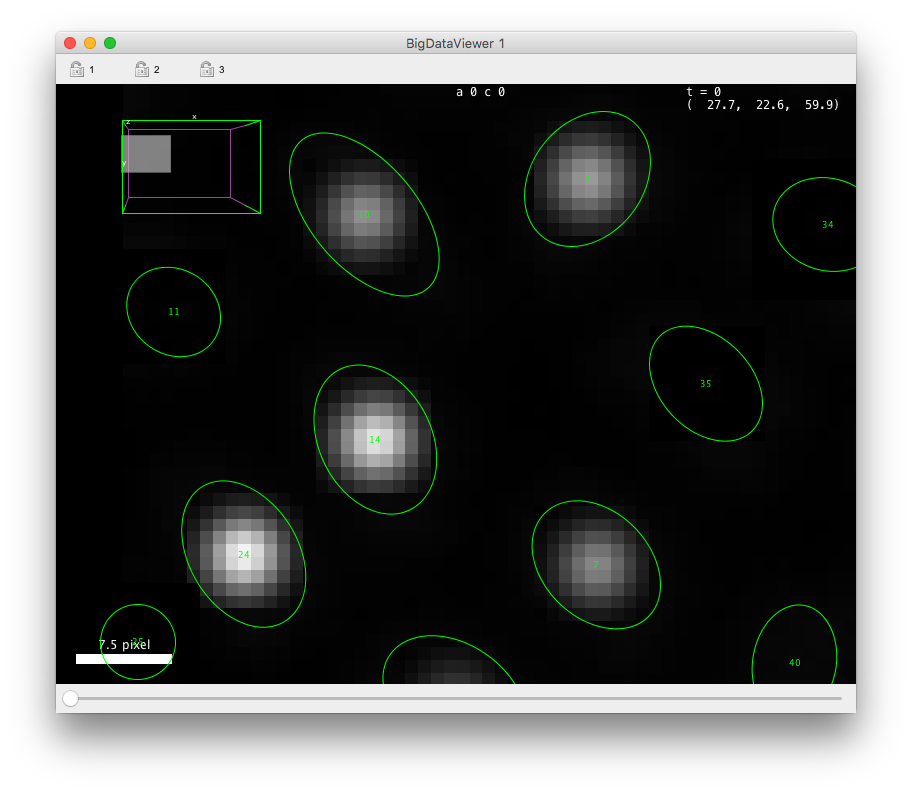
\includegraphics[width=6cm]{figures/Mastodon_GaussMeanIntensityWeights.png}
    \caption{Illustration of the Gaussian weights used in the \textbf{Spot gaussian-filtered intensity} feature.}
    \label{fig:SpotGaussWeights}
\end{figure}
    
\subsubsection{Spot median intensity.}

There is one projection of this feature per channel.
It reports the median intensity in the center of the spot for each channel.
The median is calculated inside a box that fits in the smallest radius of the ellipsoid.
The Figure~\ref{fig:SpotMedianBox} illustrates what this box looks like for several spots.

\begin{figure}
    \centering
    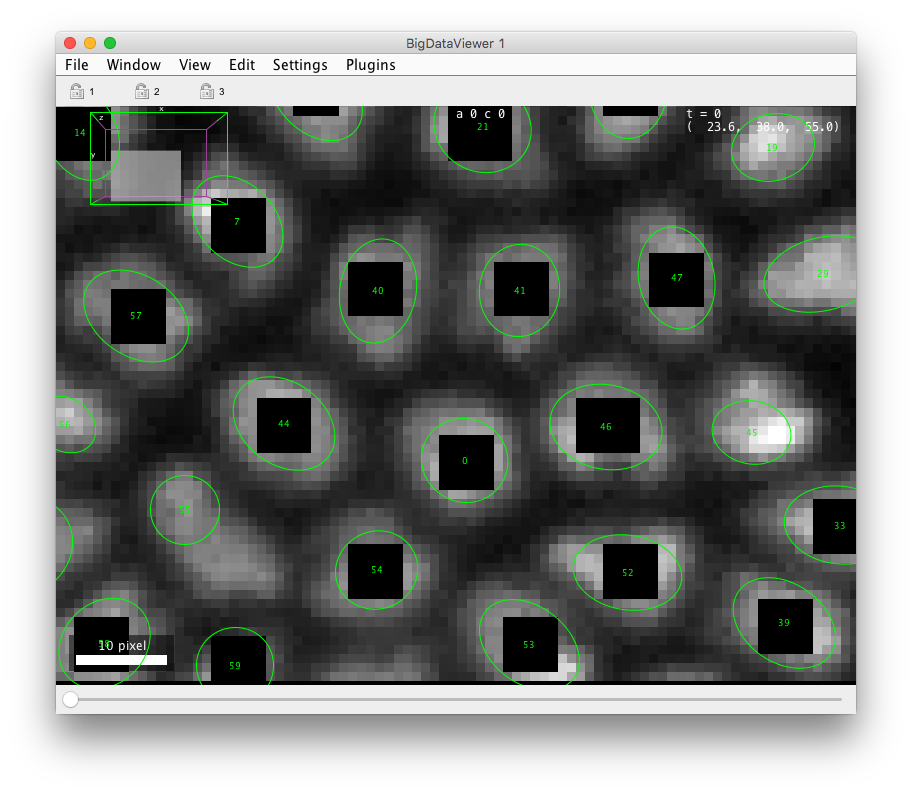
\includegraphics[width=6cm]{figures/Mastodon_Median-feature-pixels.png}
    \caption{Illustration of the box in which the \textbf{Spot median intensity} feature is calculated.}
    \label{fig:SpotMedianBox}
\end{figure}

\subsubsection{Other spot features.}
{
\footnotesize

\begin{tabular}{p{0.17\textwidth}|p{0.17\textwidth}|p{0.57\textwidth}}

    \toprule
    \textbf{Feature name} &
    \textbf{Projections} &
    \textbf{Description}             
    \\ \midrule
    
    \multicolumn{2}{l|}{Spot frame} & 
    The spot frame.
    \\ \midrule

    \multicolumn{2}{l|}{Spot N links} & 
    The total number of links, incoming and outgoing, of the spot.
    \\ \midrule
    
    Spot position &
    X, Y, Z &
    The spot center position, in physical units.
    \\ \midrule
    
    \multicolumn{2}{l|}{Spot radius} & 
    The spot radius in physical units. 
    
    For spots that are ellipsoids, returns a radius using the geometric mean of the spot ellipsoid radiuses. This approximation is such that the sphere with the reported radius and the spot ellipsoid have the same volume.
    \\ \midrule
    
    Spot sum intensity & 
    One value per channel &
    The total spot intensity for all the pixels inside the spot ellipsoid.
    \\ \midrule
    
    \multicolumn{2}{l|}{Spot track ID} &
    The ID of the track the spot belongs to.
    Track IDs are positive integer numbers starting from 0.
    \\ \midrule

\end{tabular}
}

\subsection{Link features.}

\subsection{Track features.}